\chapter{Literature Review}

\section{Cardiac Diffusion MRI}

Magnetic Resonance Imaging (MRI) is the imaging method that was used to acquire the data on which are results are based. It is non-invasive and especially adapted to soft-tissues. \cite{bakermans2008} We will explain briefly how it works and what information it gives us.

\subsection{Physics of MRI}

Magnetic Resonance acquisitions rely on the physical properties of the body, and more specifically the most abundant nucleus which is hydrogen (H). Indeed water molecules represent more than 70\% of the entire body composition. This hydrogen nucleus consists of 1 proton and 1 electron of opposite electrical charge. The relative position of the electron in respect to the proton leads to different electron spin that is a property of this atom and makes it behave like a magnetic dipole. Applying an external magnetic field $\mathbf{B_0}$ leads to a precession around the direction of $\mathbf{B_0}$ of the nuclear magnetic moment of the nucleus. Its magnetic moment will have a characteristic frequency $\omega_0$. All the magnetic moments of the nuclei in a specific region will average out to a net magnetization vector $\mathbf{M_0}$ aligned with $\mathbf{B_0}$.\\
Then the idea is to apply a secondary and much less intense magnetic field $\mathbf{B_1}$, with $||\mathbf{B_1}|| \simeq 10^{-6}||\mathbf{B_0}||$ in a direction in the plane orthogonal to the direction of $\mathbf{B_0}$, rotating around the direction of $\mathbf{B_0}$ with the Larmor frequency $\omega_0$ to bring the nuclei out of their equilibrium and into an excited state. This can be achieved by transmitting radio frequency (RF) pulses.\\

\subsection{At the service of Imaging}

Once the nuclei are in its excited state, its relaxation and the outcome magnetization vector in the $(x, y)$ plane $\mathbf{M_{x, y}}$ induces a current recorded by a RF receiving coil. This is the signal that is measured in a MR experiment and that will be used to acquire the data.\\
For acquisitions in 2D or 3D there are gradient applied to the RF pulse depending on the location, so that the receiving coil can differentiate more easily depending on this modulation. Typically in 2D for a slice they use frequency and phase encoding for the 2 degrees of freedom. In 3D slice selection is accomplished via a linear magnetic gradient, so that the main exterior magnetic field $\mathbf{B_0}(z)$ is different for each slice and leads to different Larmor values for each value of $z$.\\
In our case all MRI are acquired ex-vivo, which means that the acquisition process is more simple as the subject is perfectly still and several acquisitions can be performed without having to worry about the subject's motion. More advanced techniques are invoked such as FLASH imaging to solve these extra requirements.

\section{Diffusion Tensor Imaging}

Magnetic resonance diffusion tensor imaging (DTI) is a method based on MRI and the diffusion mechanism of water molecules to assess the direction of fibers from the anisotropic property of the diffusion of these molecules in a structure that contains boundaries.\\

\subsection{Physical diffusion property of molecules}

In general the DTI signal is based on the proton of the hydrogen nucleus present in water molecules.\\
In a non-restrictive volume, the motion of molecules also called Brownian motion has a Gaussian distribution at equilibrium that is linked to the temperature of the environment and other properties of this environment. This Gaussian distribution will be deviated in the presence of physical barriers that will decrease the diffusivity. Indeed molecules' motion will be hindered in the direction perpendicular to the obstacles. When barriers are present the diffusion will change from isotropic to anisotropic. If we look at a free water molecule, its diffusion would be in the shape of a sphere whereas with boundaries the diffusion of the same water molecule would be more of an ellipsoid with principal direction orthogonal to the boundary.

\subsection{Applied to diffusion weighted imaging}

Two short and intense successive pulsed field gradients (PFGs) are applied to the region of interest. The first makes protons have a precession phase proportional to their position along the direction of the gradient. Then a second one is applied with the exact opposite direction so that molecules that didn't move will have a precession phase null whereas those that moved will have a precession phase proportional to their motion in the direction of the PFG. Here we talk about single water molecules but in reality we are considering distribution of water molecules, and for unbounded water molecules the distribution will be centered around a null motion whereas bounded ones will have a motion distribution centered around the direction orthogonal to the main boundary.

\subsection{To get a diffusion tensor matrix}

Diffusion anisotropy can be described mathematically by a 3x3 diffusion tensor:
\begin{equation}
    \mathbb{D} = \begin{pmatrix}
    D_{xx} & D_{xy} & D_{xz} \\
    D_{yx} & D_{yy} & D_{yz} \\
    D_{zx} & D_{zy} & D_{zz}
    \end{pmatrix}
\end{equation}

with $D_{ij}$ the apparent diffusion coefficient (ADC) in direction $(i, j)$. $\mathbb{D}$ is symmetric, which means that $D_{ij} = D_{ji}$.\\
In conclusion we need at least 6 independent gradient directions to determine all 6 degrees of freedom in this matrix. In practice 7 directions are used to get more accurate results, along with a non-weighted measurement.\\
The values that we analyze most frequently are ADC and fracional anisotropy (FA):
\begin{equation}
    ADC = \frac{tr{\mathbb{D}}}{3} = \frac{\lambda_1 + \lambda_2 + \lambda_3}{3}
\end{equation}
\begin{equation}
    FA = \sqrt{\frac{(\lambda_1 - \lambda_2)^2 + (\lambda_2 - \lambda_3)^2 + (\lambda_3 - \lambda_1)^2}{\lambda_1^2 + \lambda_2^2 + \lambda_3^2}}
\end{equation}

\section{Fiber modeling}

We are using Maurer-Cartan description of fibers geometry in our study of heart fibers. \cite{pami2015, savadjiev2012heart, piuzephd, levy1935methode} Indeed the heart fiber structure is a dense and continuous set that we want to model in the best way possible. The Maurer-Cartan method provides good descriptors of smooth manifolds in $\mathbb{R}^3$, using a moving frame. This method of moving frame combined with a minimal surface model and the Generalized Helicoidal model (GHM) can efficiently characterize heart fiber geometry.

\subsection{Theory of moving frames}

We utilize the framework described in \cite{de1990ventricular} to describe the geometry of fiber orientation in the heart wall via rotations of a frame field that is fit to the diffusion MRI data. \\
Let a point $\mathbf{x} = \sum_i{x_i\mathbf{e_i}} \in \mathbb{R}^3$ be expressed in terms of $(\mathbf{e_1}, \mathbf{e_2}, \mathbf{e_3})$, the natural basis for $\mathbb{R}^3$. \\
We define a right-handed orthonormal frame field $\mathbf{f_1},\mathbf{f_2},\mathbf{f_3} : \mathbb{R}^3 \to \mathbb{R}^3$. \\ 
Each frame axis can be expressed by the rigid rotation $f_i = \sum_i{a_{i,j}\mathbf{e_j}}$, where $\mathbf{A} = {a_{i,j}} \in \mathbb{R}^{3 \times 3}$ is a differentiable attitude matrix such that $\mathbf{A}^{-1} = \mathbf{A}^T$. \\
Treating $\mathbf{f_i}$ and $\mathbf{e_j}$ as symbols, we can write:
\begin{equation}
\begin{bmatrix}
    \mathbf{f_1} \\
    \mathbf{f_2} \\
    \mathbf{f_3}
\end{bmatrix} = \mathbf{A} \times \begin{bmatrix}
    \mathbf{e_1} \\
    \mathbf{e_2} \\
    \mathbf{e_3}
\end{bmatrix}
\end{equation}

Since each $\mathbf{e_i}$ is constant, the differential geometry of the frame field is completely characterized by $\mathbf{A}$. Taking the exterior derivative on both sides, we have:
\begin{equation} \label{eq:1}
\begin{split}
    \partial \begin{bmatrix}
                \mathbf{f_1} \\
                \mathbf{f_2} \\
                \mathbf{f_3}
            \end{bmatrix} &= (\partial \mathbf{A})\mathbf{A}^{-1}  \begin{bmatrix}
                \mathbf{f_1} \\
                \mathbf{f_2} \\
                \mathbf{f_3}
            \end{bmatrix} \\
            &= \mathbf{C}
            \begin{bmatrix}
                \mathbf{f_1} \\
                \mathbf{f_2} \\
                \mathbf{f_3}
            \end{bmatrix}
\end{split}
\end{equation}
where $\partial$ denotes the exterior derivative, and $\mathbf{C} = (\partial \mathbf{A}) \mathbf{A}^{-1} = (c_{i,j}) \in \mathbb{R}^{3 \times 3}$ is the Maurer-Cartan matrix of connection forms $(c_{i,j})$. \\
Writing $\mathbf{f}_i$ as symbols, \ref{eq:1} is to be understood as $\partial \mathbf{f}_i = \sum_j{c_{i,j}\mathbf{f}_j}$. \\
The Maurer-Cartan matrix is skew symmetric with zeros as diagonal entries so there are at most 3 independent, non-zero 1-forms: $c_{1,2}$, $c_{1,3}$, and $c_{2,3}$. \\
1-forms operate on tangent vectors through contraction, written as $\partial \omega \langle \boldsymbol{\upsilon} \rangle \in \mathbb{R}$ for a general 1-form $\partial \omega = \sum_i{\omega_i \mathbf{e_i}}$ and tangent vector $\boldsymbol{\upsilon} \in \mathbb{R}^3$, which yields:
\begin{equation}
\begin{split}
    \partial \omega \langle \boldsymbol{\upsilon} \rangle &= \sum_i{\omega_i \partial \mathbf{e_i}} \big{\langle} \sum_j{\upsilon_j \mathbf{e_j}} \big{\rangle} \\
    &= \sum_i{\omega_i \upsilon_i}
\end{split}
\end{equation} since $\partial \mathbf{e_i} \langle \mathbf{e_j} \rangle = \delta_{i,j}$, where $\delta_{i,j}$ is the Kronecker delta. \\
It turns out that the space of linear models for smoothly varying frame fields is parametrized by the 1-forms $c_{i,j}$. Since only 3 unique non-zero combinations of $c_{i,j}$ are possible, there are in total 9 connections $c_{i,j,k}$. These coefficients express the rate of turn of the frame vector $\mathbf{f}_i$ towards $\mathbf{f}_j$ when $\mathbf{x}$ moves in the direction $\mathbf{f}_k$. 

\subsection{Application to heart fiber geometry}

With $\mathbf{f}_1$ taken as the local orientation of a fiber and $\mathbf{f}_3$ taken to be the component of the heart wall normal orthogonal to $\mathbf{f}_1$, \ref{fig:c123theory} illustrates the connection $c_{1,2,3}$, which measures the rotation of fibers for a trans-mural penetration of the wall.\\

\begin{figure}[h]
    \centering
    \begin{subfigure}[t]{.48\textwidth}
        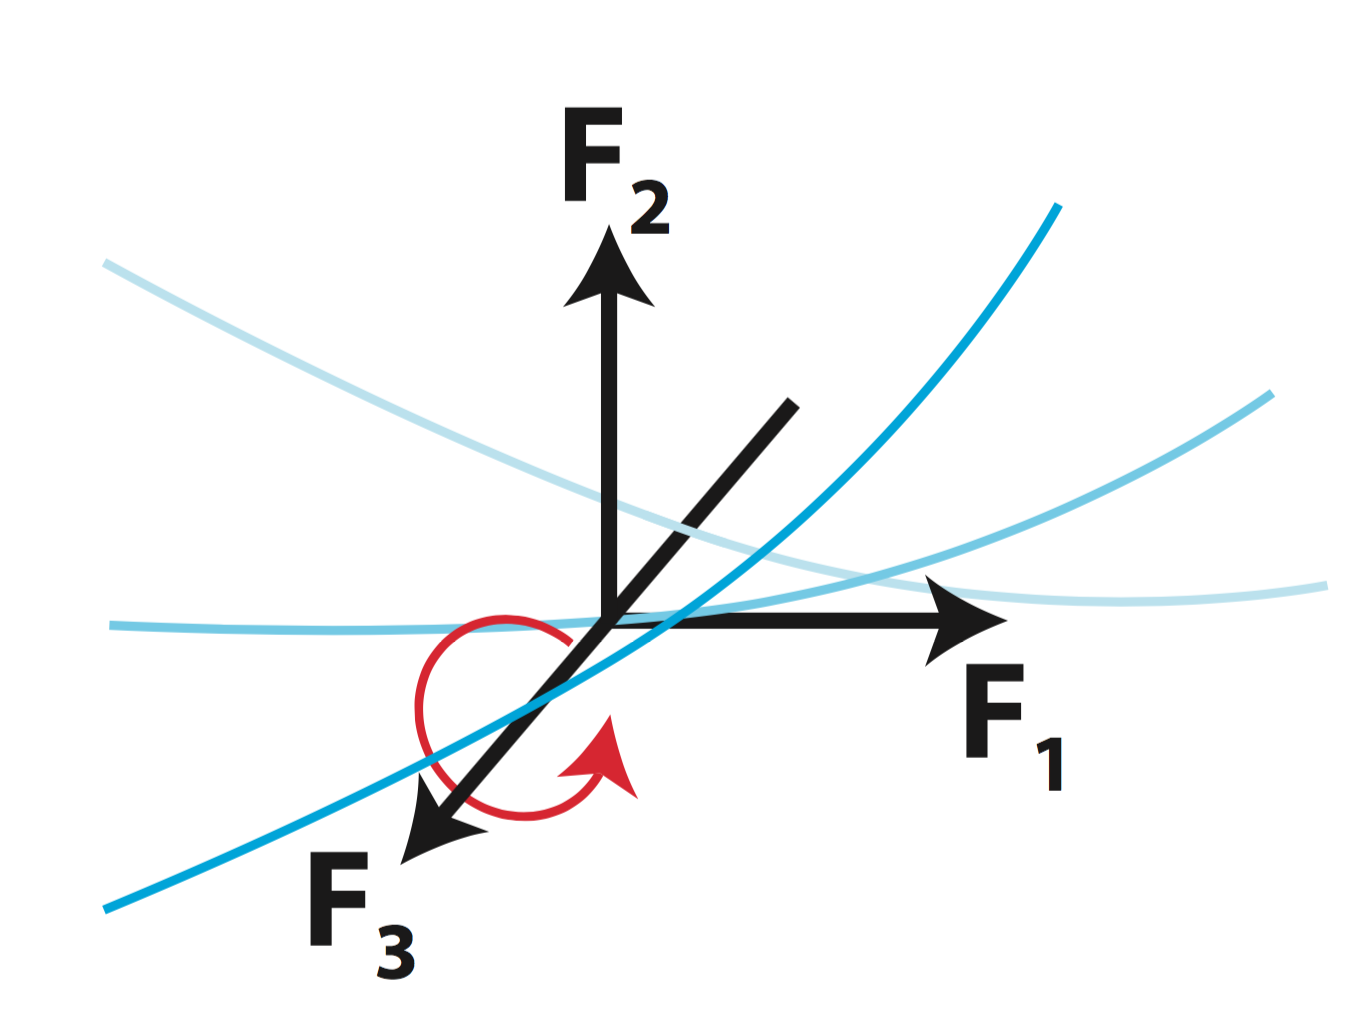
\includegraphics[width=\textwidth]{figures/c123}
        \caption[b]{Geometry evolving as we move in the direction of $\mathbf{F_3}$, with the color getting more intense as we move out of plane}
        \label{fig:c123}
    \end{subfigure}
    \begin{subfigure}[t]{.48\textwidth}
        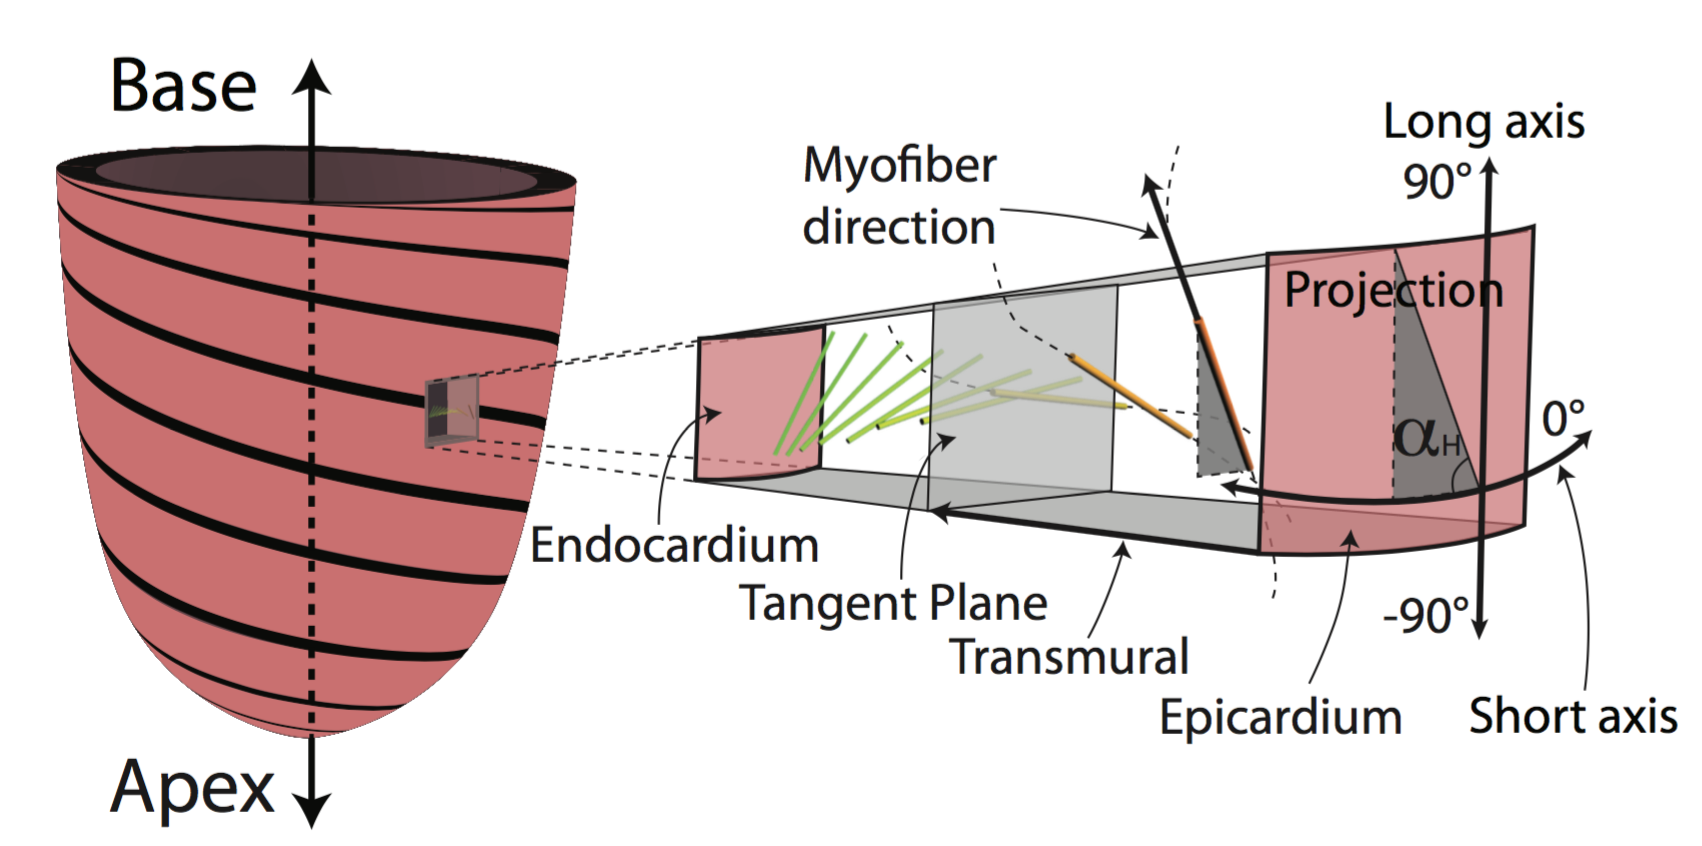
\includegraphics[width=\textwidth]{figures/helix_angle}
        \caption{Most significant rotation the heart we will focus on}
        \label{fig:helix_angle}
    \end{subfigure}
    \caption{Signification of Maurer-Cartan forms, and more specifically $c_{1,2,3}$ in the chosen configuration on heart data}
\end{figure}

\section{Infarcts and their impact on heart fiber geometry}

\cite{pmbpop2013quantification, mediamihaela}